\chapter{Architectural Design}

\section{Overview}
The CKB platform system is composed by a 3-tier architecture.\\
Its software application architecture is organized into three logical tiers: the presentation tier, or user interface; the application tier, where data is processed; and the data tier, where the data associated with the application is stored and managed.

\begin{figure}[H]
    \centering
    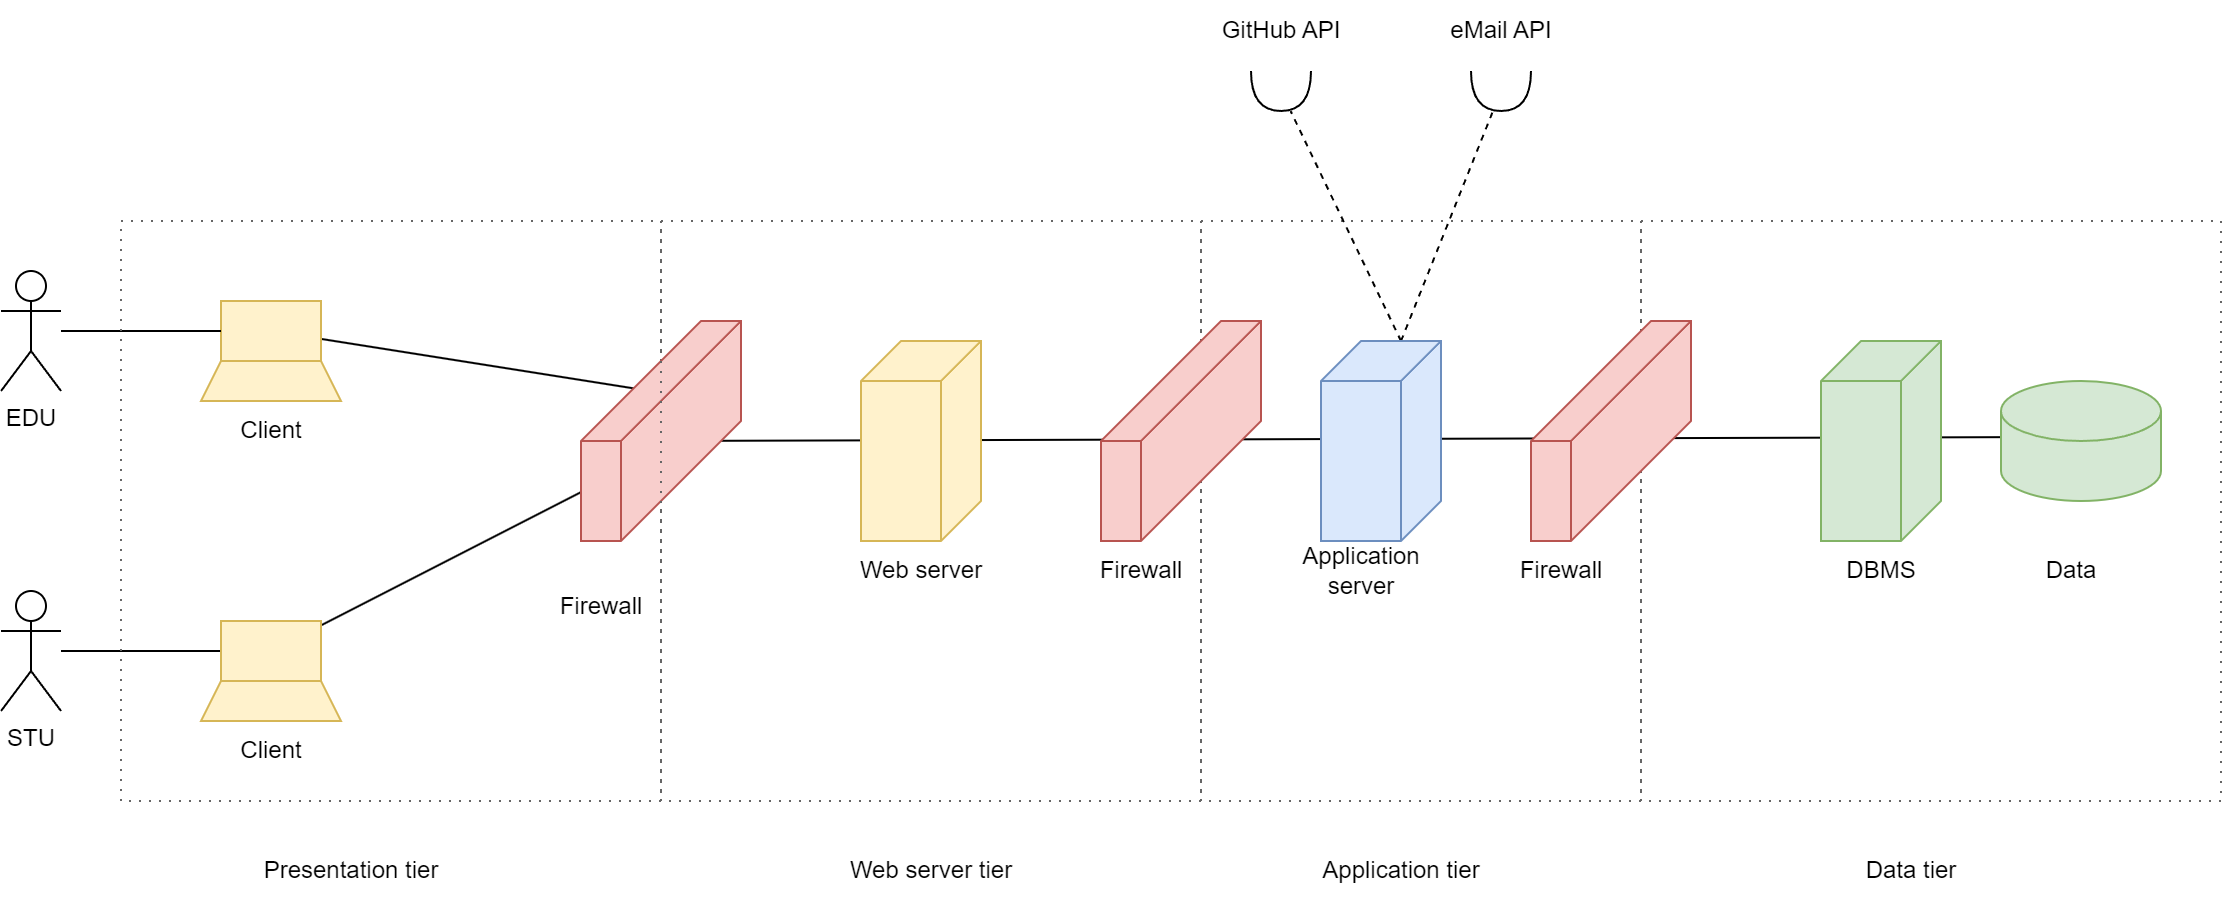
\includegraphics[width=\textwidth]{images/diagrams/high_level_diagram.png}
    \caption{High level components diagram}
\end{figure}

{\color{red} qui i load balancer è un errore metterli? \\ Qualcosa mi fa pensare che debba mettere sia web server che application server, ma non sono sicuro}

The service will be accessed through a web interface, employing a Single Page Application (SPA). Utilizing an SPA is ideal for this application, as it facilitates extensive interaction without necessitating frequent page reloads.\\
The system's architecture is structured into distinct layers, with application servers interacting with a database management system and utilizing APIs for data retrieval and storage. {\color{red}Adhering to REST standards, the application servers are intentionally designed to be stateless, -e le sessioni di log in come ce le gestiamo?-} while the system will include more than one firewall to ensure security.\\

\section{Component view}
The system is composed by the following components:

\begin{figure}[H]
    \centering
    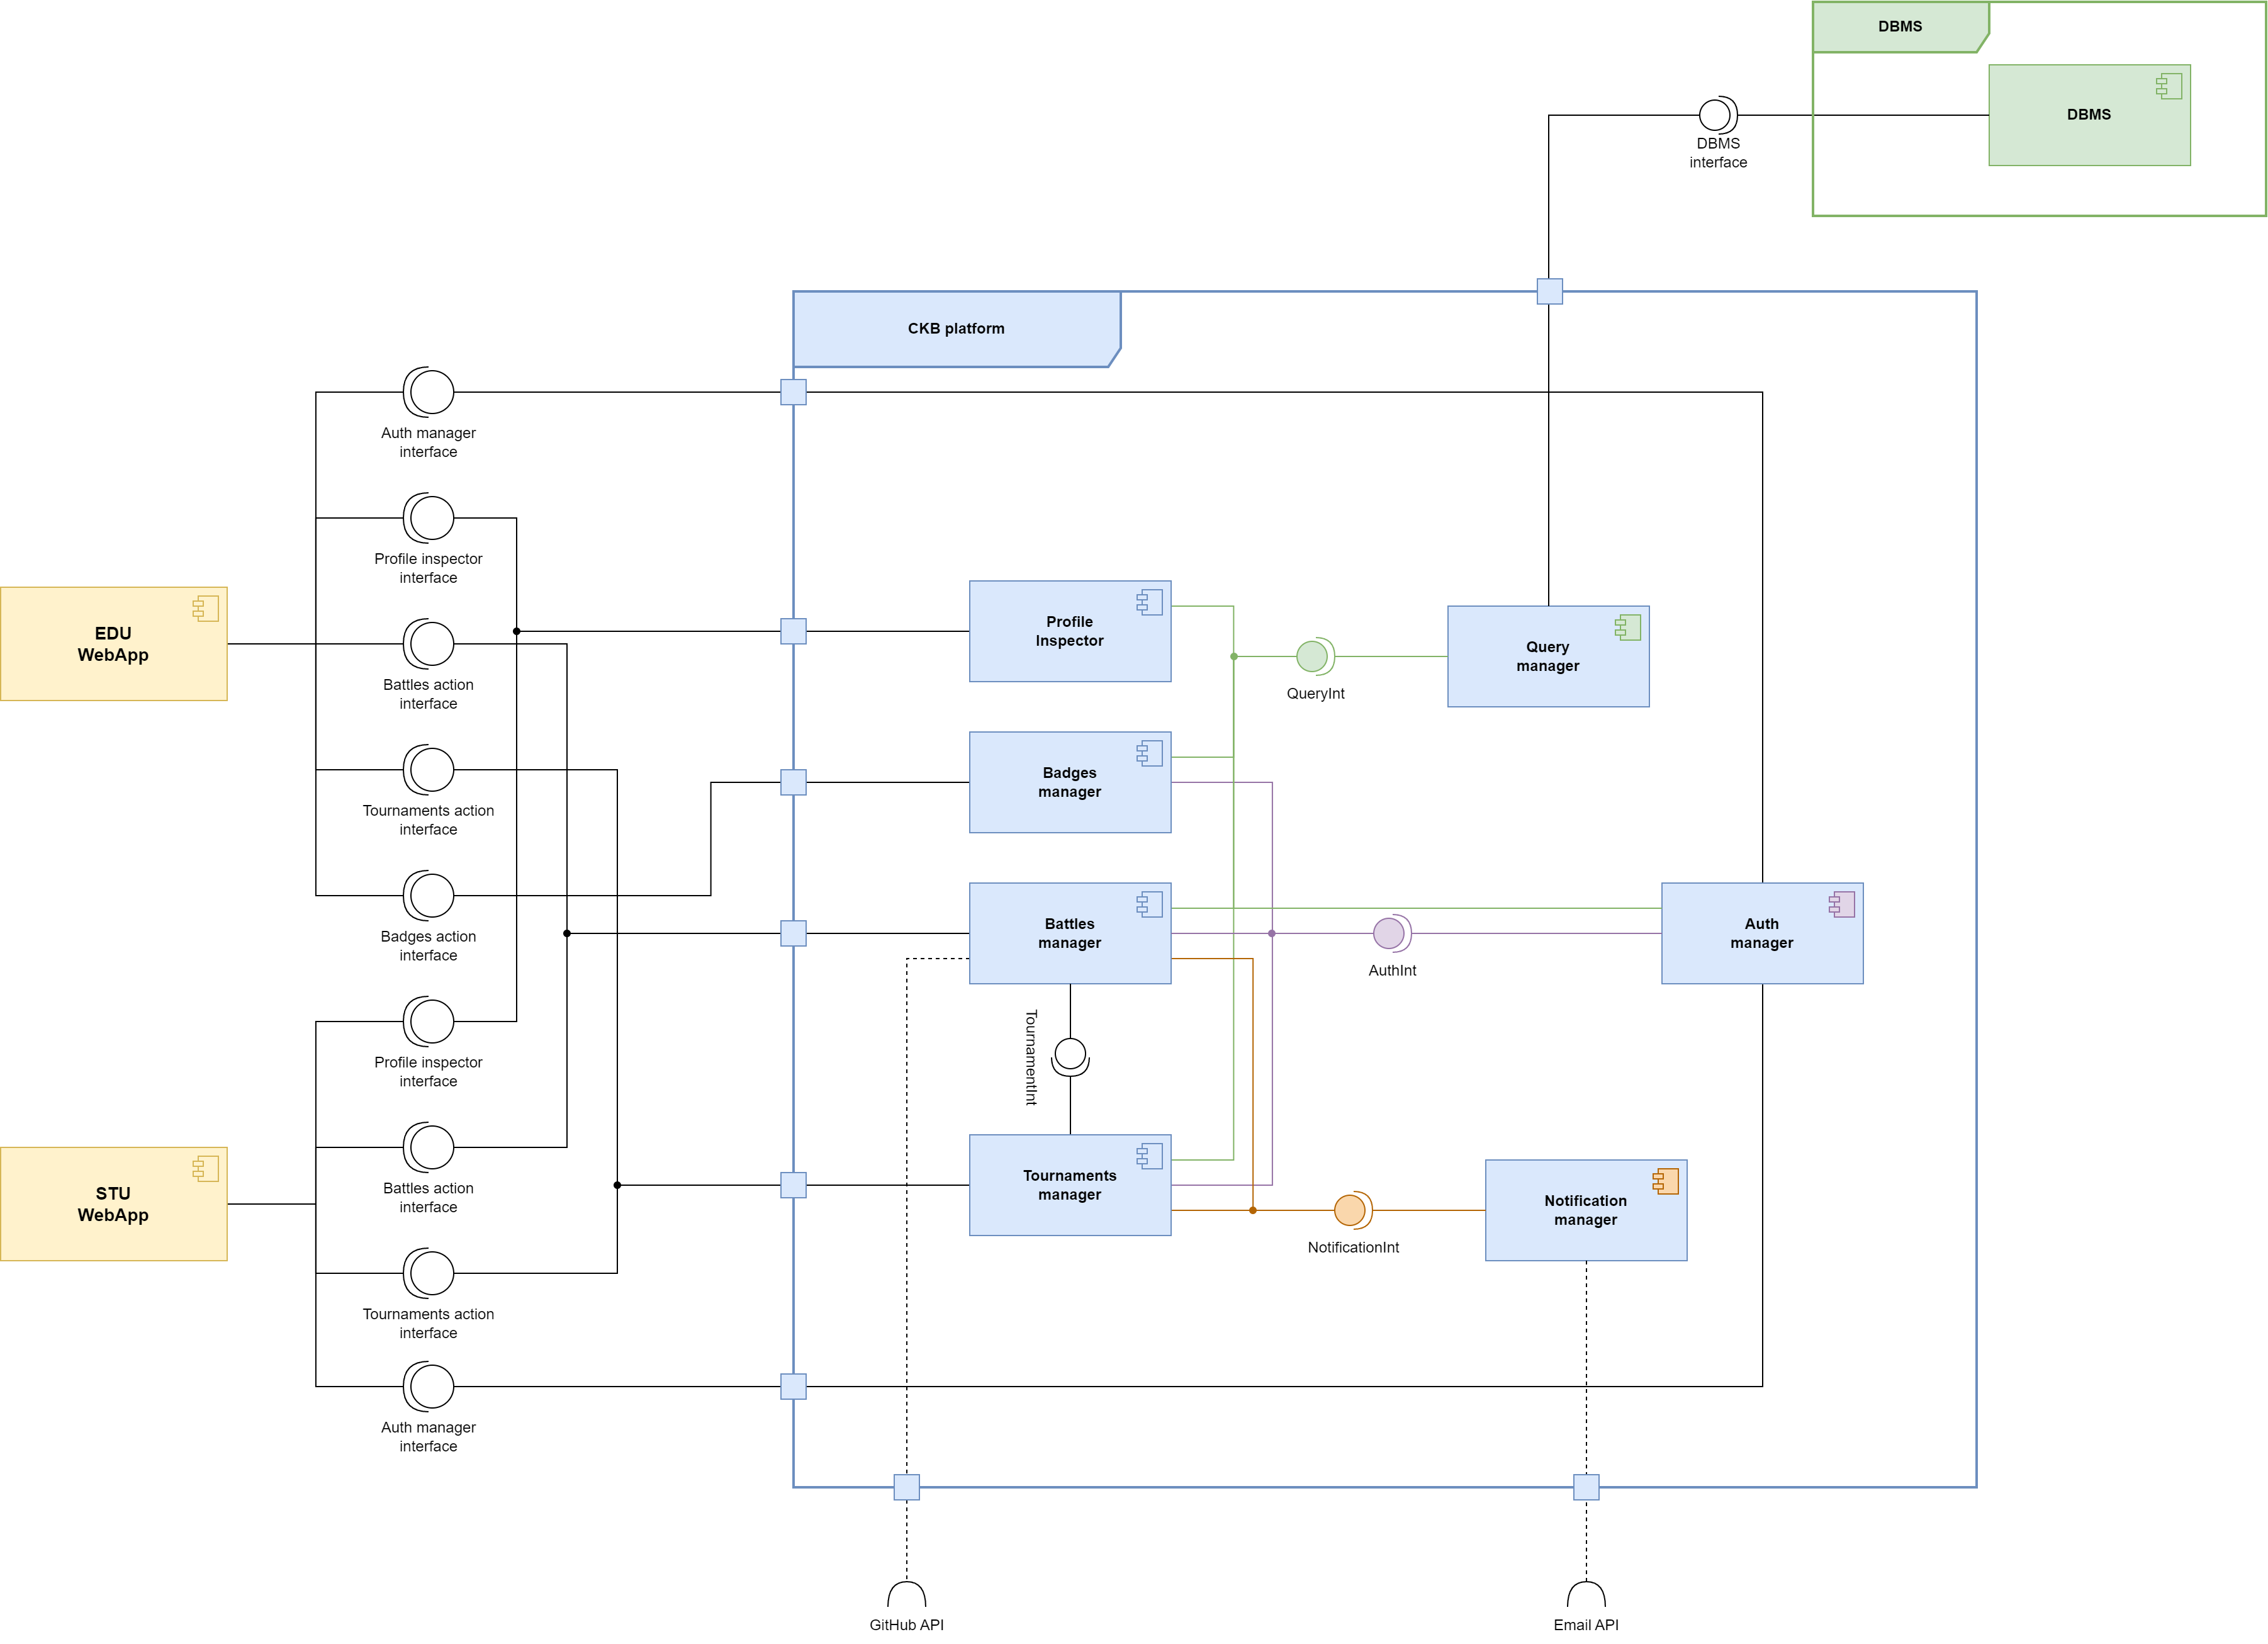
\includegraphics[width=\textwidth]{images/diagrams/component_diagram.png}
    \caption{Component diagram}
\end{figure}

{\color{red}Qui va bene aver raggruppato le interfacce oppure vanno messe singolarmente, una per ogni endpoint?}

\subsection{Client components}

The client components are represented by only a single component, a user-friendly WebApp, that will behave differently depending on the level of the user that is using it (whether it is an EDU or a STU).\\
The WebApp is interfaced with the server components through all the APIs offeded by the server (see later for a detailed description of the APIs).\\
{\color{red}Vogliamo aggiungere come mai abbiamo scelto di fare una WebApp e non un'applicazione mobile?}

\subsection{Server components}

\subsubsection*{Query manager}
The query manager is the component that handles the queries made by the other components that need to access the database. It is responsible for the execution of the queries and for the communication with the database.\\
It is interfaced with all the internal models of the system that need to access the database, i.e. all the other components of the system exept for the notification manager.\\
It is interfaced with the database through the DBMS API, external to the system.

\subsubsection*{Auth manager}
The auth manager is the component that handles the authentication of the users and the authorization of the requests made by the other components that need to access the database with respect to the user that made the request.\\
It is interfaced with all the internal models of the system that behave differently depending on the level of the user that made the request, i.e. the badges manager, the tournament manager and the battle manager.\\
It isn't interfaced with any external component.

\subsubsection*{Notification manager}
The notification manager is the component that handles the need of the system to notify the users of some events, such as the start of a tournament or the end of a battle.\\
It is interfaced with all the internal models of the system that need to notify the users, i.e. the tournament manager and the battle manager.\\
It is interfaced with the Email API, external to the system.

\subsubsection*{Badges manager}
The badges manager is the component that handles the gamification badges.\\
It allows:
\begin{itemize}
    \item the creation of new badges;
    \item the assignment of badges to the STUs;
    \item the visualization of the badges assigned to a user (?)
\end{itemize}
{\color{red}Qui devo interfacciare anche con battle e user?}
It is interfaced with the auth manager (since the creation of a badge is admissible only for the EDUs) and with the query manager (since it needs to access the database to store the badges).\\
It is interfaced with the EDU WebApp through the proprer, external to the system.

\subsubsection*{Tournaments manager}
The tournament manager is the component that handles the management of the tournaments.\\
It allows:
\begin{itemize}
    \item the creation of new tournaments;
    \item the closure of the torunaments
    \item the visualization of the tournaments;
    \item the excange of admin permission between EDUs;
    \item the subscription of the STUs to the tournaments;
    \item the visualization of the scores of the EDUs in the tournaments, and so of the ranking
\end{itemize}
It is interfaced with the auth manager (to allow and perform different actions depending on the level of the user that made the request), with the query manager (since it needs to access the database) and the notification manager (since it needs to notify the users of the start and the end of a tournament).\\
It is interfaced with the WebApp, both EDU and STU, through the proper APIs, external to the system.

\subsubsection*{Battles manager}
The battles manager is the component that handles the management of the battles.\\
It allows:
\begin{itemize}
    \item the creation of new battles;
    \item the subscription of the STUs to the battles;
    \item the visualization of the scores of the teams in the battles, and so of the ranking
    \item the visualization of the battles;
    \item the automatic evaluation of the battles;
    \item the eventual manual evaluation of the battles by the EDUs
\end{itemize}
It is interfaced with the auth manager (to allow and perform different actions depending on the level of the user that made the request), with the query manager (since it needs to access the database) and the notification manager (since it needs to notify the users of the opening of subscriptions, the start and the end of a bettle).\\
It is interfaced with the WebApp, both EDU and STU, through the proper APIs and with GitHub (to perform the manual evaluation), all external to the system.

\subsubsection*{Profile Inspector}
The profile inspector is the component that handles the visualization of the profiles of the STUs and, consequently, of the badges that a STU has earned during the battles and the tournaments.\\
It is interfaced with the query manager (since it needs to access the database).
It is interfaced with the WebApp, both EDU and STU, through the proper APIs, external to the system.

\subsection{Logical description of the data}
The data of the system is organized in a relational database, with the following entity-relationship diagram:

\begin{figure}[H]
    \centering
    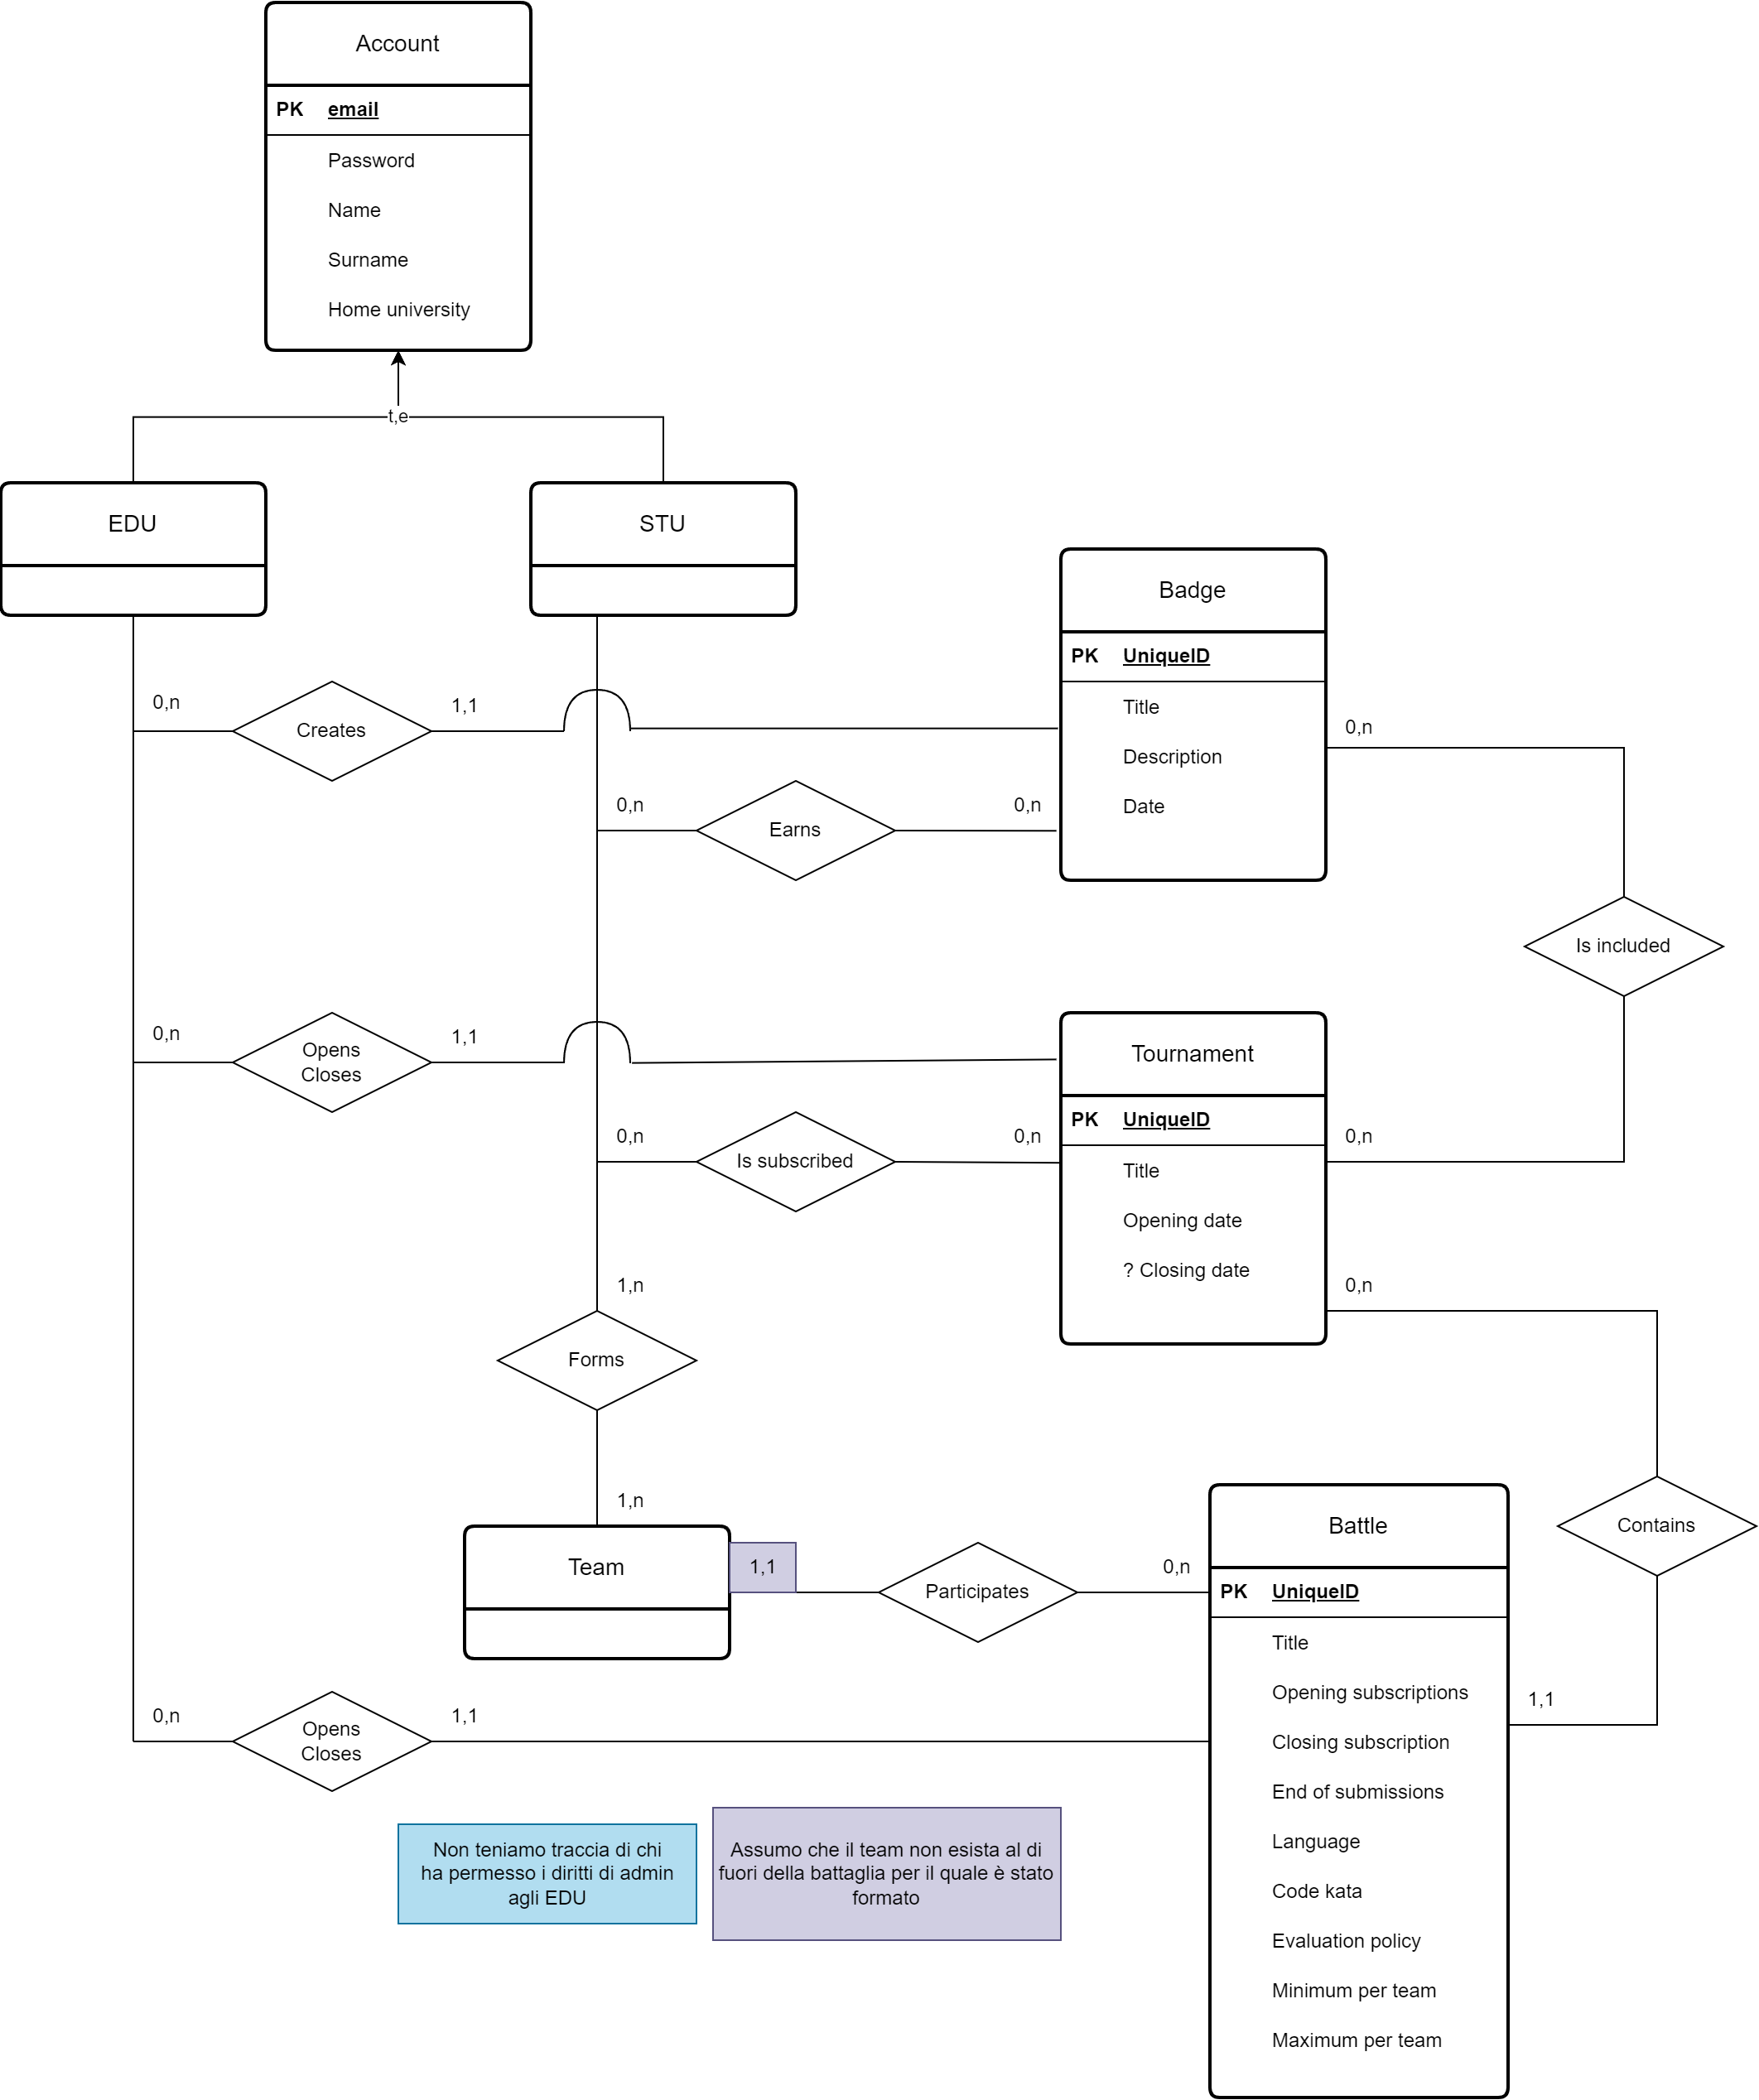
\includegraphics[width=0.75\textwidth]{images/diagrams/er_diagram.png}
    \caption{Entity-relationship diagram}
\end{figure}

\section{Deployment view}
Our system comprises two essential components: a static web server and an application server. The static web server serves as the entry point for clients to access the SPA, while the application server furnishes the necessary APIs for the SPA's functionality. To optimize performance, we have opted for distinct solutions for these components.\\
The static web server will be hosted on a CDN (Content Delivery Network) on cloud, exploiting its edge location caches and reverse proxies to ensure rapid response times. On the other hand, the application server, containing both a business logic layer and a data tier, will find its home on a cloud provider. This decision offers numerous advantages over traditional in-house hosting, including:
\begin{itemize}
    \item \textbf{Scalability and Flexibility}: The cloud infrastructure allows for the dynamic addition or removal of resources like virtual machines, performance cores, or memory as per the evolving needs. Load balancing services further enable the application server to adapt seamlessly to changes in traffic or workload.
    \item \textbf{Security}: Enhanced security features, such as live monitoring and firewalls, contribute to safeguarding the application server against potential data breaches, cyberattacks, and other security threats.
    \item \textbf{Cost-efficiency}: The cloud provider's pay-as-you-go model ensures cost efficiency by charging only for the utilized resources. This approach helps in reducing overall costs, making it a financially prudent choice.
\end{itemize}
These attributes position a cloud provider as an ideal hosting solution for large, high-traffic applications. The selected cloud provider must respect all these features to effectively meet our system requirements.\\
